\documentclass[10pt,twocolumn]{article}

\usepackage[margin=0.72in]{geometry}
\setlength{\columnsep}{0.24in}
\usepackage{times}
\usepackage[round,authoryear]{natbib}
\usepackage{microtype}
\usepackage{graphicx}
\usepackage{booktabs}
\usepackage{tabularx}
\usepackage{multirow}
\usepackage{amsmath,amssymb,mathtools}
\usepackage{enumitem}
\usepackage{xcolor}
\usepackage{hyperref}
\usepackage[capitalize,noabbrev]{cleveref}
\usepackage{caption}
\usepackage{subcaption}
\usepackage{array}
\usepackage{pifont}

\hypersetup{
  colorlinks=true,
  linkcolor=blue!55!black,
  citecolor=green!35!black,
  urlcolor=blue!55!black
}
\captionsetup{font=small,labelfont=bf}
\setlength{\parindent}{1em}
\setlength{\parskip}{0pt}
\setlist{leftmargin=*,nosep}
\setlength{\textfloatsep}{8pt plus 2pt minus 2pt}
\setlength{\floatsep}{7pt plus 2pt minus 2pt}
\setlength{\intextsep}{7pt plus 2pt minus 2pt}
\emergencystretch=2em

\newcommand{\todo}[1]{\textcolor{red!75!black}{\textbf{[TODO: #1]}}}
\newcommand{\todoexp}[1]{%
  \par\noindent\textcolor{red!75!black}{\textbf{TODO experiment.} #1}\par}
\newcommand{\todoplot}[1]{%
  \par\noindent\textcolor{red!75!black}{\textbf{TODO figure/result.} #1}\par}
\newcommand{\direct}{\textsc{Direct}}
\newcommand{\enumplain}{\textsc{Enum}}
\newcommand{\enumindex}{\textsc{Index-Enum}}
\newcommand{\native}{\textsc{Native-CoT}}
\newcommand{\R}{\mathbb{R}}
\newcommand{\ind}{\mathbb{I}}
\newcommand{\eps}{\varepsilon}
\newcommand{\softmax}{\operatorname{softmax}}
\newcommand{\logit}{\operatorname{logit}}
\newcommand{\Var}{\operatorname{Var}}
\newcommand{\E}{\mathbb{E}}
\newcommand{\KL}{\operatorname{KL}}
\newcommand{\cmark}{\ding{51}}
\newcommand{\xmark}{\ding{55}}

\title{\vspace{-1.2em}\textbf{From Global Aggregation to Sequential Retrieval:\\
How Chain-of-Thought Changes Long-Context Counting}}
\author{Anonymous Authors}
\date{}

\begin{document}
\maketitle
\vspace{-1.2em}

\begin{abstract}
Counting sparse, semantically defined records in a long context requires at least two operations:
retrieving the relevant records and aggregating how many were found.
We study how language models implement these operations under direct answering, explicit
enumeration, indexed enumeration, and native chain-of-thought (CoT).
Our working hypothesis is an \emph{algorithmic path switch}: direct answering relies primarily on
a broad, normalized aggregation followed by a noisy global numerosity readout, whereas explicit
reasoning decomposes the task into sequential targeted retrieval and a trace-local accumulator.
We formalize the distinction at three levels---behavior, representations, and causal circuits---and
specify falsifiable criteria for calling an internal state a counter or an attention head a functional
retrieval component. Preliminary realistic NIAH experiments show large gains from native thinking
and explicit enumeration, but also substantial model-by-mode and query-order interactions.
The final paper will combine a broad behavioral panel, causal analyses of Qwen and Gemma,
and training-dynamics experiments in controlled synthetic transformers.
\todo{Replace this hypothesis-level abstract with measured effect sizes and the final causal conclusion.}
\end{abstract}

\section{Introduction}
Language models can solve difficult reasoning problems while failing to count a small number of
relevant objects embedded in a long prompt. This failure is not a single primitive deficit.
A model may fail to identify all relevant records, may retrieve them but aggregate them incorrectly,
may encode the correct count in a representation that the output pathway cannot read, or may stop
or format its response incorrectly. Counting in a needle-in-a-haystack (NIAH) setting therefore
offers a controlled probe of how retrieval, memory, and arithmetic interact.

A natural intervention is to ask the model to reason explicitly. In our pilot experiments,
native thinking and explicit enumeration substantially improve exact counting on Qwen and Gemma.
However, improved accuracy alone does not establish a mechanism. CoT may change which records are
retrieved, externalize a latent state, provide convenient numeric tokens, alter the stopping policy,
or merely select a different decoding path. Our goal is to determine \emph{which computation changes}
and to connect that change causally to count error.

Recent work already establishes that counting is a nontrivial transformer computation.
Small-model studies characterize multiple learned counting algorithms
\citep{golkar2024contextual,chang2025inductive,behrens2025counting};
large-model studies report latent count states, layerwise counters, structured System-2
decomposition, and geometric readout bottlenecks
\citep{hasani2026understanding,hasani2026system2,garcia2026direction}.
Our setting differs in two ways. First, the relevant items are sparse semantic records dispersed
among distractors rather than a homogeneous repeated list or externally partitioned input.
Second, we compare the same unstructured context across direct and explicit-reasoning paths,
allowing us to test whether CoT changes the underlying \emph{retrieval-and-aggregation algorithm}.

The intended contribution is a causal account with four parts:
\begin{enumerate}
    \item a controlled behavioral map over count $N$, context length $L$, reasoning mode,
    query order, model family, and failure type;
    \item an evidence hierarchy separating count decodability, dynamic counter consistency,
    and causal use of a count state;
    \item an operational and causal taxonomy of broad aggregation, targeted retrieval,
    and progress-transition components; and
    \item a bridge from synthetic training dynamics to functional motifs in open-weight LLMs.
\end{enumerate}
The central claim will be promoted only if the interventions support it.
In particular, we do \emph{not} assume in advance that direct answering contains a clean running
counter, nor that an attention heatmap alone identifies a causal head.

\begin{figure*}[t]
    \centering
    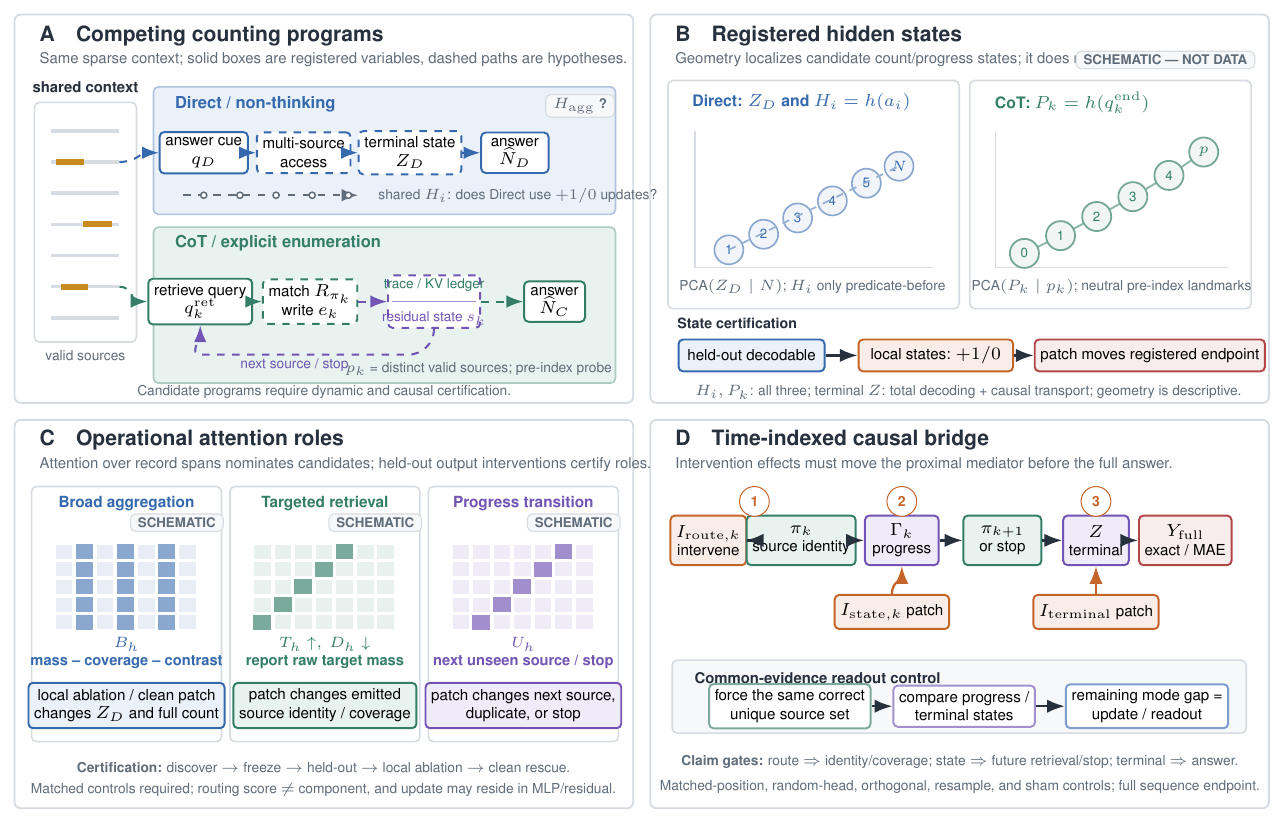
\includegraphics[width=\textwidth]{figures/mechanism_overview.png}
    \caption{\textbf{Proposed analysis and claim boundary.}
    Direct answering is tested against two alternatives: a causally used running counter and a
    delayed global aggregation/readout. Explicit reasoning is tested for sequential targeted
    retrieval and a trace-local accumulator. PCA is only visualization; held-out decoding,
    dynamic consistency, and interventions form the evidence ladder. Head labels require a
    selective causal effect and negative controls. Panel D states the required causal bridge from
    retrieval or state interventions to final count error. The diagram is schematic, not data.}
    \label{fig:overview}
\end{figure*}

\section{Task and Experimental Factors}
\subsection{Sparse-record counting}
A prompt contains a sequence of $L$ tokens $x_{1:L}$ encoding $R$ records and distractor text.
Record $r$ occupies a token span $I_r=[s_r,e_r]$. A query defines a predicate
$\psi_q(r)\in\{0,1\}$, and the gold set and count are
\[
    G_q=\{r:\psi_q(r)=1\},
    \qquad N=|G_q|.
\]
For token-level analyses we use a canonical landmark $a_r$, normally the final content token or
delimiter immediately after record $r$. The cumulative semantic count at position $t$ is
\[
    c_q(t)=\sum_{r:e_r\le t}\psi_q(r).
\]
This definition is independent of any number printed in the model's trace.

We vary count $N$, canonical context length $L$, record positions, record identities, distractor
content, and query order $o\in\{\text{query-first},\text{query-last}\}$ while reusing matched
stimuli across modes and models.

\subsection{Reasoning modes}
We distinguish four interfaces:
\begin{description}[style=nextline,font=\normalfont\scshape]
    \item[\direct] Return only the final count.
    \item[\enumplain] List the matching records without numeric indices, then return a total.
    \item[\enumindex] List the matching records with explicit indices $1,2,\ldots$, then return a total.
    \item[\native] Use the model's native visible reasoning mode and return a final count.
\end{description}
The unindexed mode is essential: a probe at an explicit token ``$k$'' can trivially decode $k$,
so indexed traces cannot by themselves establish an internal accumulator.

Let $\hat N$ denote the parsed final count. Primary behavioral metrics are exact accuracy,
absolute error $|\hat N-N|$, signed error $\hat N-N$, parse success, truncation, and protocol
compliance. For explicit enumeration we additionally parse the retrieved multiset
$\widehat G$ and report unique recall, false positives, duplicates, and aggregation errors.

\subsection{Two-tier model panel}
The behavioral panel is intentionally broader than the mechanism panel.
\begin{table*}[t]
\centering
\small
\begin{tabularx}{\textwidth}{p{0.18\textwidth}X X}
\toprule
Panel & Models & Purpose and claim scope \\
\midrule
Behavior / empirical law &
Qwen family at approximately 4B, 8B, 14B, and 32B; Gemma4-E4B;
GLM-4-9B and GLM-Z1-9B; Cogito-v1-8B; Nemotron-Nano-v2-9B;
Nemotron-3-Nano-4B &
Estimate mode effects, degradation with $N$ and $L$, family heterogeneity, and failure budgets.
Within-family curves are primary; cross-family pooled slopes are secondary. \\
Mechanism &
Qwen-8B and Gemma4-E4B &
Full hidden-state capture, attention and head-output analysis, steering, activation patching,
path patching, ablation, and matched negative controls. \\
Synthetic dynamics &
Small causal transformers under the finalized v15/v20-style task &
Track when performance, representations, routing motifs, and causal effects emerge during training. \\
\bottomrule
\end{tabularx}
\caption{Planned model organization. Exact checkpoint identifiers, tokenizer revisions, chat
templates, and active/total parameter counts must be frozen in the final protocol.}
\label{tab:modelpanels}
\end{table*}

\todoexp{Freeze exact checkpoint IDs and decoding templates. Do not treat a nominal parameter
count as a clean scaling variable across dense and mixture-of-experts families.}

\section{Behavioral Map Before Mechanism}
\subsection{Paired evaluation and failure decomposition}
All mode comparisons use identical stimuli and are paired within
(model, $N$, $L$, seed, query order). Exact accuracy is computed on all requests, with parse
failures, truncations, and formatting failures retained as failures. We separately report
conditional numerical accuracy among successfully parsed outputs to avoid conflating counting
with interface compliance.

For enumeration outputs, define
\[
\begin{aligned}
 \mathrm{FN} &= |G_q\setminus \operatorname{uniq}(\widehat G)|,\\
 \mathrm{FP} &= |\operatorname{uniq}(\widehat G)\setminus G_q|,\\
 \mathrm{Dup} &= |\widehat G|-|\operatorname{uniq}(\widehat G)|.
\end{aligned}
\]
When the reported total is the list length plus an arithmetic/protocol residual $A$,
\[
    \hat N-N = \mathrm{FP}-\mathrm{FN}+\mathrm{Dup}+A.
\]
This decomposition distinguishes retrieval failure from a correct list followed by a wrong total.

\todoplot{Main behavioral figure: a grid of exact-accuracy and mean-absolute-error surfaces over
$(N,L)$ for \direct, \enumplain, \enumindex, and \native, with Qwen and Gemma highlighted.
Use paired bootstrap intervals clustered by stimulus.}

\todoexp{Run $N\in\{1,\ldots,10,20,30\}$ and at least three canonical context lengths with
five or more seeds. Preserve query-first and query-last as a factorial variable rather than
collapsing it: current pilots show large mode-by-order interactions.}

\subsection{Empirical response surfaces, not a forced universal law}
Because current pilot fits are unstable across architectures, the main paper should not depend on
a single universal scaling law. Let $Y_i=\ind\{\hat N_i=N_i\}$. A defensible hierarchical model is
\[
\begin{aligned}
\logit\,\Pr(Y_i=1)
&=\alpha_{f(i),m(i),o(i)}\\
&\quad+f_{f(i),m(i)}
      \bigl(\log L_i,\log(N_i+1)\bigr).
\end{aligned}
\]
where $f$ denotes model family, $m$ reasoning mode, and $o$ query order. Candidate response
surfaces include linear, log-linear, interaction, and shape-constrained smooth models.
Model selection is performed by held-out stimulus clusters using log loss and Brier score, not
in-sample $R^2$. Signed and absolute errors are modeled separately.

\todoexp{Pre-register the candidate function class and a grouped train/validation/test split.
Promote a quantitative law only if it improves held-out prediction over a condition-only baseline
and its coefficients are stable under seed and template perturbations. Otherwise report monotone
qualitative degradation with uncertainty.}

\subsection{Expected behavioral statement}
The target statement is:
for moderate contexts and $N\le 10$, native CoT and the two enumeration modes are close and
substantially outperform direct answering; all modes degrade as $N$ and $L$ increase, and absolute
error increases. This statement must be qualified by model family, query order, truncation budget,
and enumeration fidelity.

\todoplot{Replace the preceding target statement with estimates and confidence intervals.
Include an appendix panel for every attempted model. For models with severe format or truncation
failure, report both intent-to-treat accuracy and a failure-budget table rather than simply calling
them ``unevaluable.''}

\section{What Counts as an Internal Counter?}
Let $h^{(\ell,m)}_t\in\R^d$ be the residual-stream state at layer $\ell$, token $t$, and mode $m$.
We use three nested evidence levels.

\paragraph{Level 1: count-decodable representation.}
There exists a decoder $g_\ell$ trained on disjoint prompts such that
$g_\ell(h_t)\approx c_q(t)$ or $N$. This establishes information availability only.

\paragraph{Level 2: dynamically consistent counter state.}
At matched landmarks, decoded state increments after a relevant record and remains invariant after
a distractor:
\[
\begin{aligned}
 \E[g_\ell(h_{a_{r+1}})-g_\ell(h_{a_r})\mid \psi_q(r+1)=1]&\approx 1,\\
 \E[g_\ell(h_{a_{r+1}})-g_\ell(h_{a_r})\mid \psi_q(r+1)=0]&\approx 0.
\end{aligned}
\]
The test must control for absolute position, relative position, record identity, total $N$,
context length, and density $N/L$.

\paragraph{Level 3: causally used counter state.}
Replacing or steering the candidate state changes downstream progress and final count in the
predicted direction, with norm-matched random, orthogonal-direction, position-matched, and sham
patch controls.

We reserve the term \emph{counter} for a state satisfying all three levels.
PCA trajectories are useful visualizations but are not evidence of a counter by themselves.

\subsection{Where to analyze direct answering}
For \direct, the primary landmarks are the original-context record endpoints $a_r$ and matched
distractor endpoints in the \emph{same forward pass}. These positions test a running state.
The final query/answer-prefix state tests a global numerosity readout. A probe that decodes $N$
only from the final state across prompts cannot distinguish a running counter from delayed
parallel aggregation.

We therefore compare two explicit hypotheses:
\begin{description}[style=nextline]
\item[$H_{\mathrm{run}}$:] A causally used cumulative state is updated at each relevant record.
\item[$H_{\mathrm{agg}}$:] Local ordinal information may be present, but the task-relevant count
is formed mainly by a later global aggregation/readout at the answer query.
\end{description}

\todoexp{At each original-context needle landmark, jointly decode
$c_q(t)$, total $N$, remaining count $N-c_q(t)$, $t$, $t/L$, and $N/L$.
Use residualized or multi-task probes and report conditional generalization to unseen
$(N,L)$ cells. This prevents position or density from masquerading as a counter.}

\todoexp{Construct clean/corrupt pairs by swapping one relevant record with a distractor while
holding $L$, record positions, and surface statistics fixed. Patch the candidate landmark state
from count $j+\Delta$ into a recipient at count $j$ and test whether later landmarks and the final
answer shift by $\Delta$.}

\subsection{Where to analyze explicit reasoning}
For \enumplain, \enumindex, and \native, define semantic progress
\[
    p_k=\left|\bigcup_{u\le k}\operatorname{uniq}(\widehat G_u)\cap G_q\right|,
\]
the number of distinct gold records retrieved by trace step $k$. Candidate accumulator landmarks
are neutral separators or the state immediately \emph{before} a numeric index is emitted.
Analyses at the printed index token are reported only as a leakage control.

\todoexp{Run three anti-leakage controls: unindexed enumeration, random nonnumeric labels, and
permuted visible indices. A genuine trace-local accumulator should track semantic progress $p_k$
and survive these controls; a token-copy explanation should not.}

\subsection{Geometry, noise, and separability}
For a fixed semantic count $c$, define the mean state and within-count covariance
\[
\begin{aligned}
  \mu_{\ell,m}(c)
  &=\E[h^{(\ell,m)}_t\mid c_q(t)=c],\\
  \Sigma_{\ell,m}(c)
  &=\operatorname{Cov}\!\left(
      h^{(\ell,m)}_t\mid c_q(t)=c
    \right).
\end{aligned}
\]
After learning a count subspace $U_\ell$ on a training split, define normalized decoding noise
\[
  \nu_{\ell,m}(c)=
  \E\!\left[
  \left(g_\ell(U_\ell^\top h_t)-c\right)^2
  \,\middle|\,c_q(t)=c
  \right].
\]
We will report between-count separation relative to within-count dispersion, not only PCA plots.

\todoplot{For each mechanism model, show layerwise 2D/3D geometry at matched landmarks,
held-out $R^2$ or classification accuracy, within-count dispersion, adjacent-count margin,
and performance split by correct versus incorrect outputs. Expected: direct states become more
overlapping as count grows; explicit-reasoning landmarks form cleaner ordered trajectories.}

\section{Operational Attention and Circuit Taxonomy}
Let $A^{(\ell,a)}_{q,s}$ be the attention weight of head $(\ell,a)$ from query position $q$ to
source position $s$. Let $\mathcal{G}$ be gold record landmarks, $g_k$ the next unvisited gold
record at trace step $k$, and $\mathcal{V}_k$ the visited gold landmarks.

For a head and query, define total gold mass, target selectivity, duplicate mass, and effective
coverage:
\[
\begin{aligned}
 M_{\mathcal G}(q)&=\sum_{s\in\mathcal G}A_{q,s},\\
 S_k(q)&=\frac{A_{q,g_k}}{M_{\mathcal G}(q)+\eps},\\
 D_k(q)&=\sum_{s\in\mathcal V_k}A_{q,s},\\
 C_{\mathcal G}(q)&=\exp\!\left(
 -\sum_{s\in\mathcal G}\tilde A_{q,s}\log(\tilde A_{q,s}+\eps)
 \right),
\end{aligned}
\]
where $\tilde A$ is attention renormalized over $\mathcal G$.

\paragraph{Broad aggregation component.}
At the final query, it places substantial total mass on many gold records
(high $M_{\mathcal G}$ and high $C_{\mathcal G}$) without selecting one record.
Its head-output ablation or patching changes the global numerosity readout.
We prefer \emph{broad aggregation} to \emph{broad retrieval}: direct errors may occur despite
recoverable needle information.

\paragraph{Targeted retrieval component.}
At trace step $k$, it concentrates on the next unvisited gold record
(high $S_k$, low $D_k$). Head-output patching must change which record is emitted or restored,
not merely the final logits.

\paragraph{Progress-transition or update component.}
Its output causally changes the next retrieval target or the trace-local progress state.
We use the term \emph{successor head} only if the OV circuit implements a token-independent
ordered map $k\mapsto k+1$ under relabeling, consistent with the stricter notion in
\citet{gould2023successor}. Otherwise ``progress-transition'' is the safer functional label.

A head role is accepted only when
\[
\begin{aligned}
&\text{observational signature}\\[-1mm]
&\quad+\text{selective causal effect}\\[-1mm]
&\quad+\text{negative controls}
\end{aligned}
\]
all agree. Attention heatmaps nominate candidates; they do not establish function
\citep{zhang2024patching}.

\todoplot{Main circuit figure: for Qwen-8B and Gemma4-E4B, show one broad-aggregation map from
the final query, one targeted-retrieval map at trace step $k$, and one progress-transition map.
Alongside each heatmap, show head-output patching and matched-ablation effect sizes.}

\todoexp{Use a discovery/test split over prompts and seeds. Discover candidate heads on one split;
freeze the head set and thresholds; evaluate necessity and sufficiency on held-out prompts.
Include random-head, same-layer, lexical-adjacency, and attention-mass-matched controls.}

\section{Causal Interventions}
\subsection{Geometric steering}
For a count direction $v_\ell$ learned only on training prompts, intervene at a selected landmark:
\[
    h'^{(\ell)}_t=h^{(\ell)}_t+\alpha v_\ell.
\]
A mechanistically meaningful direction should produce a monotone, localized change in decoded
progress and final count over an interval of $\alpha$, while norm-matched random and orthogonal
directions should not. Steering that merely changes verbosity or digit preference is insufficient.

\subsection{Activation and path patching}
For clean prompt $x^+$ and matched corrupt prompt $x^-$, patch a state or head output
$z$ from clean into corrupt. Let
\[
 \Delta_{\mathrm{logit}}(x)
 =\log p(\text{gold count}\mid x)
 -\log p(\text{corrupt count}\mid x).
\]
A normalized restoration score is
\[
 \operatorname{Rest}(z)=
 \frac{\Delta_{\mathrm{logit}}(x^-;z\leftarrow z^+)
       -\Delta_{\mathrm{logit}}(x^-)}
      {\Delta_{\mathrm{logit}}(x^+)-\Delta_{\mathrm{logit}}(x^-)}.
\]
We additionally evaluate semantic outcomes: selected record, unique retrieval recall, progress
state, stopping point, and final count.

\subsection{Necessity, sufficiency, and mediation}
Mean or resample ablation tests necessity; clean-to-corrupt patching tests partial sufficiency.
To connect the two algorithmic layers, interventions must change a retrieval/update metric and
that change must predict the count change.

\todoexp{Estimate the mediated path
intervention $\rightarrow$ targeted-retrieval fidelity $\rightarrow$ progress-state accuracy
$\rightarrow$ final count. Report direct and mediated effects with prompt-cluster bootstrap
intervals; do not infer mediation from cross-sectional correlations alone.}

\section{A Noise Model Connecting Mechanism to Error}
\subsection{Direct normalized aggregation}
A minimal hypothesis for direct answering is a normalized pooled representation
\[
    r=\sum_{t=1}^L a_t v_t,\qquad \sum_t a_t=1.
\]
If relevant and distractor tokens receive relative weight ratio $1:\alpha$, then a scalar
relevance statistic can behave approximately as
\[
    \rho(N,L)
    =\frac{N}{N+\alpha(L-N)}+\eta,
\]
where $\eta$ is representation and routing noise. Inverting the noiseless map gives
\[
    N(\rho,L)
    =\frac{\alpha L\rho}{1-(1-\alpha)\rho},
    \qquad
    \frac{\partial N}{\partial\rho}
    =\frac{\alpha L}
    {[1-(1-\alpha)\rho]^2}.
\]
Thus a small error in a normalized density-like code can be amplified by context length.
This model is a falsifiable explanation for increasing absolute error; it is not assumed true.

\todoexp{Fit density, magnitude, and running-counter hypotheses on held-out prompts.
Compare predictive likelihood and intervention responses. Test whether final-query states encode
$N/L$ more stably than $N$, whether the inverse-readout slope predicts absolute error, and whether
needle-attention denominator manipulations change the count as predicted.}

\subsection{Sequential targeted retrieval}
Under idealized stepwise retrieval, exact success can be decomposed as
\[
\begin{aligned}
\Pr(\text{exact})
&\approx \Pr(\text{protocol succeeds})\\
&\quad\times
\prod_{k=1}^{N}
\left(1-\eps_k^{\mathrm{miss}}
        -\eps_k^{\mathrm{dup}}\right.\\[-1mm]
&\hspace{7.0em}\left.
        -\eps_k^{\mathrm{fp}}\right).
\end{aligned}
\]
up to dependence and final aggregation error. CoT need not make every state noiseless; it can
improve performance by replacing one ill-conditioned global inversion with locally checkable
retrieval/update steps.

\todoexp{Measure stepwise miss, duplicate, false-positive, and stopping hazards as functions of
$k$, $N$, and $L$. Test whether targeted-head ablation increases the corresponding hazard before
it changes final count, and whether clean head-output patching rescues both.}

\section{Synthetic Training Dynamics}
The synthetic experiments are not a separate paper. Their role is to reveal when the functional
motifs arise under controlled training and to validate the intervention pipeline before applying
it to LLMs.

At checkpoint $s$, measure behavioral accuracy $A_s$, held-out count decodability $R_s$,
dynamic-consistency score $D_s$, causal patch restoration $P_s$, broad-aggregation score $B_s$,
and targeted-retrieval score $T_s$. For metric $M_s$ and threshold $\gamma$, define emergence time
\[
    \tau_\gamma(M)=\min\{s:M_s\ge\gamma\}.
\]
We ask whether decodability precedes causal use, whether targeted retrieval appears before a clean
trace-local accumulator, and whether CoT training suppresses the direct path or adds a parallel
path.

\todoexp{Use the finalized v15/v20-style synthetic setting, checkpoint densely around the behavioral
transition, and run at least three seeds. The current v10 suite can supply the causal analyses,
but architecture, tokenization, train/test count ranges, and loss masks must match the final
setting. The v20 report was not available in the material inspected for this draft; insert its
exact specification before freezing the paper.}

\todoplot{Training-dynamics figure with aligned x-axis in optimization steps or tokens:
(a) direct and CoT accuracy; (b) probe and dynamic-consistency metrics; (c) causal restoration;
(d) head-role scores. Mark emergence times and seed variability.}

\section{Main Result Logic and Decision Rules}
The paper should read as a sequence of increasingly strong claims:
\begin{enumerate}
\item \textbf{Behavior:} explicit reasoning improves sparse long-context counting under matched
stimuli, with quantified dependence on $N$, $L$, model, and query order.
\item \textbf{Representation:} count or progress information is geometrically organized, but
decodability is separated from causal use.
\item \textbf{Routing:} direct and explicit modes exhibit different functional attention motifs.
\item \textbf{Causality:} state and head interventions selectively alter retrieval/update variables
and consequently alter final count.
\item \textbf{Mechanistic bridge:} the direct path's noise or conditioning and the explicit path's
stepwise retrieval errors explain the behavioral curves.
\end{enumerate}

The following decision rules prevent overclaiming:
\begin{itemize}
\item If direct landmarks satisfy Levels 1--3, revise the story to compare a noisy internal running
counter with an externalized counter; do not force delayed aggregation.
\item If direct landmarks are decodable but patches do not propagate, describe ``available ordinal
information,'' not a used counter.
\item If explicit progress disappears under no-index or relabeling controls, restrict the claim to
targeted retrieval and numeric-token scaffolding.
\item If attention patterns are not causally selective, report routing signatures rather than a
circuit.
\item If Qwen and Gemma use different components, claim functional convergence only if the same
retrieval/update decomposition is causally supported; do not claim head-level universality.
\end{itemize}

\section{Related Work and Positioning}
\paragraph{Counting algorithms and inductive bias.}
Controlled transformer studies show that counting admits multiple mechanisms and depends strongly
on architecture, positional encoding, and optimization
\citep{golkar2024contextual,yehudai2024count,chang2025inductive,behrens2025counting}.
Our synthetic section uses training dynamics to connect these observations to LLM-scale motifs.

\paragraph{Counting in pretrained LLMs.}
\citet{hasani2026understanding} identify layerwise count states and a final-token counter on
repeated-item tasks. \citet{hasani2026system2} use externally partitioned inputs and intermediate
counts to obtain System-2 large-scale counting. \citet{garcia2026direction} identifies a geometric
readout bottleneck across several counting tasks. Our paper must explicitly distinguish these
possibilities in sparse NIAH: retrieval can be intact while global aggregation is ill-conditioned;
a readout bottleneck can coexist with routing noise; and explicit reasoning can change the
retrieval algorithm without externally partitioning the input.

\paragraph{Reasoning traces and circuits.}
CoT and scratchpads can externalize intermediate computation
\citep{nye2021scratchpad,wei2022cot}. Mechanistic work identifies recurrent motifs such as induction
and successor heads \citep{olsson2022induction,gould2023successor}, while activation patching
requires careful corruption, metrics, and controls \citep{zhang2024patching}.
We apply these standards to semantic retrieval and counting progress.

\section{Limitations}
The mechanism claims will be restricted to the tested checkpoints, prompts, and task distribution.
Native reasoning traces may be policy-dependent and need not faithfully expose all internal
computation. Attention-head identities may not be stable across seeds or model families.
The NIAH generator simplifies natural document structure, and exact count is only one form of
quantitative reasoning. Finally, interventions can be off-manifold; all steering and patching
results therefore require magnitude sweeps, resample controls, and behavioral side-effect audits.

\section{Conclusion}
The proposed paper should not be framed merely as ``CoT improves counting.''
Its defensible target is a causal account of an algorithmic change:
from a broad, normalized, globally read-out computation to sequential content-addressed retrieval
with an explicit progress state. The behavioral benchmark motivates the phenomenon; representation
geometry localizes candidate state; head analyses identify routing motifs; and interventions must
connect both to error. Whether the final evidence supports the full path-switch claim or a narrower
retrieval-only claim is left to the planned experiments.

\begin{thebibliography}{99}

\bibitem[Behrens et~al.(2025)Behrens, Biggio, and Zdeborov\'a]{behrens2025counting}
Freya Behrens, Luca Biggio, and Lenka Zdeborov\'a.
\newblock Counting in small transformers: The delicate interplay between attention and
feed-forward layers.
\newblock In \emph{ICML}, 2025. arXiv:2407.11542.

\bibitem[Chang and Bisk(2025)]{chang2025inductive}
Yingshan Chang and Yonatan Bisk.
\newblock Language models need inductive biases to count inductively.
\newblock In \emph{ICLR}, 2025. arXiv:2405.20131.

\bibitem[Garcia(2026)]{garcia2026direction}
Gabriel Garcia.
\newblock The right answer, the wrong direction: Why transformers fail at counting and how to fix it.
\newblock arXiv:2605.03258, 2026.

\bibitem[Golkar et~al.(2024)Golkar et~al.]{golkar2024contextual}
Siavash Golkar et~al.
\newblock Contextual counting: A mechanistic study of transformers on a quantitative task.
\newblock arXiv:2406.02585, 2024.

\bibitem[Gould et~al.(2023)Gould, Ong, Ogden, and Conmy]{gould2023successor}
Rhys Gould, Euan Ong, George Ogden, and Arthur Conmy.
\newblock Successor heads: Recurring, interpretable attention heads in the wild.
\newblock arXiv:2312.09230, 2023.

\bibitem[Hasani et~al.(2026a)Hasani et~al.]{hasani2026understanding}
Hosein Hasani et~al.
\newblock Understanding counting mechanisms in large language and vision-language models.
\newblock In \emph{CVPR}, 2026. arXiv:2511.17699.

\bibitem[Hasani et~al.(2026b)Hasani et~al.]{hasani2026system2}
Hosein Hasani et~al.
\newblock Mechanistic interpretability of large-scale counting in LLMs through a System-2 strategy.
\newblock arXiv:2601.02989, 2026.

\bibitem[Nye et~al.(2021)Nye et~al.]{nye2021scratchpad}
Maxwell Nye et~al.
\newblock Show your work: Scratchpads for intermediate computation with language models.
\newblock arXiv:2112.00114, 2021.

\bibitem[Olsson et~al.(2022)Olsson et~al.]{olsson2022induction}
Catherine Olsson et~al.
\newblock In-context learning and induction heads.
\newblock arXiv:2209.11895, 2022.

\bibitem[Wei et~al.(2022)Wei et~al.]{wei2022cot}
Jason Wei et~al.
\newblock Chain-of-thought prompting elicits reasoning in large language models.
\newblock In \emph{NeurIPS}, 2022.

\bibitem[Yehudai et~al.(2024)Yehudai, Kaplan, Ghandeharioun, Geva, and Globerson]{yehudai2024count}
Gilad Yehudai, Haim Kaplan, Asma Ghandeharioun, Mor Geva, and Amir Globerson.
\newblock When can transformers count to $n$?
\newblock arXiv:2407.15160, 2024.

\bibitem[Zhang and Nanda(2024)]{zhang2024patching}
Fred Zhang and Neel Nanda.
\newblock Towards best practices of activation patching in language models: Metrics and methods.
\newblock In \emph{ICLR}, 2024. arXiv:2309.16042.

\end{thebibliography}

\clearpage
\appendix
\begin{table*}[t]
\centering
\small
\begin{tabularx}{\textwidth}{p{0.07\textwidth}p{0.22\textwidth}X p{0.19\textwidth}}
\toprule
Priority & Experiment & Required controls / outputs & Claim enabled \\
\midrule
P0 & Standardized behavioral rerun &
Matched stimuli; four modes; query order; exact/MAE/signed error; parse, truncation, protocol,
retrieval and aggregation budgets; clustered intervals &
Robust phenomenon and model scope \\
P0 & Direct running-counter vs delayed-aggregation test &
Needle/distractor landmarks; joint confound probes; one-needle swap corruption; state patching;
density and position controls &
Meaning of the direct representation \\
P0 & CoT accumulator anti-leakage &
Unindexed enumeration; random labels; permuted indices; pre-number landmarks; semantic progress &
Trace-local accumulator rather than token copying \\
P0 & Qwen and Gemma causal state interventions &
Train/test split; steering sweep; clean/corrupt patching; random/orthogonal/sham controls &
Causally used count/progress state \\
P0 & Head-role validation &
Frozen discovered heads; head-output/path patching; resample ablation; random/same-layer and
attention-mass controls &
Broad aggregation and targeted retrieval functions \\
P0 & Mechanism-to-error bridge &
Stepwise hazard metrics; mediated effects; intervention-induced changes in count error &
Core algorithm-switch explanation \\
P1 & Synthetic training dynamics &
Dense checkpoints; three seeds; aligned v15/v20 final setting; emergence times &
Developmental support and methodology validation \\
P1 & Cross-model functional replication &
Same metrics and interventions in Qwen and Gemma; permit different head identities &
Functional generality \\
P1 & Query-order causal disambiguation &
Repeat instruction near generation; hold task information and recency separately &
Prompt-order mechanism rather than incidental correlation \\
P1 & Empirical-law validation &
Pre-registered candidate functions; within-family fits; grouped held-out evaluation &
Optional quantitative law \\
P2 & Transfer and broader tasks &
New record schemas, predicates, natural documents, and other aggregation tasks &
External validity \\
\bottomrule
\end{tabularx}
\caption{Concrete experiment roadmap. P0 items are necessary for an ICLR-level mechanistic claim;
P1 items substantially strengthen it; P2 items are extensions.}
\end{table*}

\section{Suggested Main-Paper Figure Order}
\begin{enumerate}
    \item Figure 1: overview and claim boundary (\cref{fig:overview}).
    \item Figure 2: paired behavioral surfaces and failure decomposition.
    \item Figure 3: direct versus CoT representation geometry with evidence ladder.
    \item Figure 4: operational head taxonomy with held-out causal effects.
    \item Figure 5: intervention $\rightarrow$ retrieval/update $\rightarrow$ count-error bridge.
    \item Figure 6: synthetic training dynamics.
\end{enumerate}

\section{Reproducibility Checklist}
The final repository should freeze model revisions, tokenizer files, chat templates, generation
parameters, random seeds, stimulus hashes, parsing code, landmark definitions, intervention hooks,
checkpoint IDs, and all discovery/test splits. Store request-level outputs rather than only
aggregates. Report GPU type, precision, batching, memory optimizations, and library versions.
For remote experiments, keep the canonical artifacts on persistent storage and mirror the
request-level tables locally.



\end{document}
